\documentclass[11pt]{article}

\usepackage[margin=1in]{geometry}
\usepackage{amsmath}
\usepackage{amssymb}
\usepackage{booktabs}
\usepackage{tabularx}
\usepackage{graphicx}
\usepackage{float}
\usepackage[round,authoryear]{natbib}
\usepackage[hidelinks]{hyperref}

% Numbers quoted in the text, written by make_figures.py.
\newcommand{\PosDiffGCTen}{0.15}
\newcommand{\PosDiffGCArcmin}{5.4}
\newcommand{\PosDiffHiArcmin}{16.9}
\newcommand{\NorthRotGCArcmin}{24}
\newcommand{\PMErrGCArcmin}{0.6}
\newcommand{\PiErrGCArcmin}{0.29}
\newcommand{\CosDecGC}{0.875}
\newcommand{\ExpansionWorst}{0.05}
\newcommand{\PMRef}{5}
\newcommand{\PiRef}{1}
\newcommand{\PMMapN}{250}
\newcommand{\PMMapDt}{10}
\newcommand{\PMMapMax}{0.066}
\newcommand{\PMMapMaxInner}{0.061}
\newcommand{\PMMapPredResid}{0.2}


\newcommand{\code}[1]{\texttt{#1}}
\newcommand{\muas}{$\mu$as}
\newcommand{\uvec}[1]{\hat{\mathbf #1}}

\title{FlyStar's tangent-plane frame and RA/Dec:\\
projection, proper motions and parallax}
\author{FlyStar development notes}
\date{Draft for discussion \\ \today}

\begin{document}
\sloppy
\maketitle

\section{Purpose}

FlyStar aligns star lists into a common frame of arcsec offsets, usually tied to
Gaia. That frame is a projection of the sky about one point. This note covers
two directions through that projection:
\begin{itemize}
  \item \emph{Into the frame} (\code{analysis.prepare\_gaia\_for\_flystar} and
    \code{analysis.project\_gaia}): Gaia positions, proper motions and
    parallaxes have to be projected consistently, with the projection
    selectable by a \code{projection='gnomonic'|'flat'|'flat\_legacy'}
    keyword (gnomonic by default).
  \item \emph{Out of the frame} (a new utility): a FlyStar \code{StarTable}'s
    fitted \code{x0}, \code{y0}, \code{vx}, \code{vy}, \code{pi} and errors
    have to be converted back to RA, Dec, $\mu_{\alpha*}$, $\mu_\delta$ and
    $\varpi$ in the same reference frame as Gaia, with arcsec offsets from a
    reference position kept alongside.
\end{itemize}
Along the way we move FlyStar's parallax reference point from the Sun to the
Solar System barycenter, as Gaia and other astrometric missions use, and add
an optional correction for the proper motions of bright Gaia stars.
For each of positions, proper motions and parallax we give the equations,
describe what FlyStar does now, and describe what we propose. Section~\ref{sec:summary}
summarizes the changes, and Section~\ref{sec:decisions} records the decisions
made and the questions still open.

\section{Conventions and reference frame}
\label{sec:conventions}

\paragraph{Sky coordinates.} Gaia DR3 \citep{Vallenari2023, Lindegren2021a}
positions $(\alpha,\delta)$ are in the ICRS \citep{Ma1998, FeisselMignard1998},
as realized by Gaia-CRF3 \citep{Klioner2022}, at the catalog reference epoch
\code{ref\_epoch} (J2016.0 for DR3). Proper motions are $\mu_{\alpha*} = \dot\alpha\cos\delta$
(\code{pmra}) and $\mu_\delta = \dot\delta$ (\code{pmdec}), and
\code{ra\_error} is already $\sigma_{\alpha*} = \sigma_\alpha\cos\delta$.

\paragraph{Unit vectors.} At a sky position $(\alpha,\delta)$ we use the
direction, local east and local north unit vectors (the normal triad
$[\mathbf p\ \mathbf q\ \mathbf r]$ of \citealt{ESA1997} and \citealt{Lindegren2012})
\begin{equation}
  \uvec u = \begin{pmatrix}\cos\delta\cos\alpha\\ \cos\delta\sin\alpha\\ \sin\delta\end{pmatrix},\qquad
  \uvec e = \begin{pmatrix}-\sin\alpha\\ \cos\alpha\\ 0\end{pmatrix},\qquad
  \uvec n = \begin{pmatrix}-\sin\delta\cos\alpha\\ -\sin\delta\sin\alpha\\ \cos\delta\end{pmatrix}.
  \label{eq:triad}
\end{equation}
These are the same vectors \code{parallax.parallax\_in\_direction} builds (as
$\uvec z\times\uvec u$ and $\uvec u\times\uvec e$). A subscript 0 means they
are evaluated at the projection center $(\alpha_0,\delta_0)$. A star's proper
motion is the rate of change of its direction,
$\dot{\uvec u} = \mu_{\alpha*}\,\uvec e + \mu_\delta\,\uvec n$, ignoring the
radial-velocity (perspective acceleration) term, which is negligible here
\citep{Butkevich2014}.

\paragraph{FlyStar's frame.} Positions are in arcsec with $+x$ toward
\emph{west} and $+y$ north, as on a detector viewed north-up. Throughout, we
write the projection in terms of east/north plane coordinates $(\xi,\eta)$ in
radians and set
\begin{equation}
  x = -\xi\,R, \qquad y = \eta\,R, \qquad
  v_x = -\dot\xi\,R, \qquad v_y = \dot\eta\,R, \qquad R = 206264.806''.
  \label{eq:xy}
\end{equation}
FlyStar fits each star's motion in this frame as
\begin{equation}
  x(t) = x_0 + v_x\,(t-t_0) + \varpi\,p_x(t), \qquad
  y(t) = y_0 + v_y\,(t-t_0) + \varpi\,p_y(t),
  \label{eq:model}
\end{equation}
where $(p_x, p_y)$ is the parallax factor (Section~\ref{sec:parallax}) and the
$\varpi$ term is present only for the Parallax motion model.

\section{Two ways to flatten the sky: flat and gnomonic}
\label{sec:projections}

A projection maps a patch of the celestial sphere onto a plane. Every
projection distorts something (lengths, angles or areas); a good choice keeps
the distortion small over the field and matches how the data were measured.
FlyStar uses one of two.

\subsection{Flat (scaled equirectangular)}

The flat projection treats RA and Dec as if they were Cartesian, scaling the RA
offset by $\cos\delta_0$ at the center so that the scale there is right:
\begin{align}
  \text{forward:}\quad &\xi_\mathrm{f} = (\alpha-\alpha_0)\cos\delta_0, & \eta_\mathrm{f} &= \delta-\delta_0, \label{eq:flat}\\
  \text{inverse:}\quad &\alpha = \alpha_0 + \xi_\mathrm{f}/\cos\delta_0, & \delta &= \delta_0 + \eta_\mathrm{f}. \label{eq:flatinv}
\end{align}
Geometrically, this lays a grid of RA and Dec onto the plane as straight,
perpendicular lines, equally spaced. The properties that follow from that:
\begin{itemize}
  \item Lines of constant RA (meridians) are parallel vertical lines, so a
    star's local north is exactly $+y$ everywhere. On the sky, meridians
    converge toward the pole.
  \item The east--west scale is right only at $\delta_0$; at another declination
    one arcsec of true east--west separation spans $\cos\delta_0/\cos\delta$
    arcsec in $\xi_\mathrm{f}$. The map is not conformal: small circles on the
    sky become ellipses away from $\delta=\delta_0$.
  \item Great circles (including the straight-line path of a star moving at
    constant proper motion, over short times) are not straight lines.
  \item It is not what a camera records, so the alignment's polynomial
    transformations must absorb the difference (Section~\ref{sec:magnitude}).
\end{itemize}
This is what \code{prepare\_gaia\_for\_flystar} and \code{project\_gaia}
use today. In map-projection terms it is the equidistant cylindrical
(equirectangular) projection with standard parallel $\delta_0$
\citep[][Sect.~12]{Snyder1987}. It is not a standard FITS WCS projection: FITS
\code{CAR} with a reference point off the equator rotates the sphere first and
gives a different (oblique) map \citep{Calabretta2002}.

\subsection{Gnomonic (tangent plane)}

The gnomonic projection places a plane tangent to the celestial sphere at
$(\alpha_0,\delta_0)$ and projects each star onto it along the line from the
center of the sphere \citep{Snyder1987}. With
$\Delta\alpha = \alpha-\alpha_0$, the standard coordinates
\citep{Green1985, Kovalevsky2004} are
\begin{equation}
\begin{gathered}
  \xi  = \frac{\uvec u\cdot\uvec e_0}{\uvec u\cdot\uvec u_0} = \frac{\cos\delta\,\sin\Delta\alpha}{D}, \qquad
  \eta = \frac{\uvec u\cdot\uvec n_0}{\uvec u\cdot\uvec u_0} = \frac{\sin\delta\cos\delta_0 - \cos\delta\sin\delta_0\cos\Delta\alpha}{D}, \\
  D = \uvec u\cdot\uvec u_0 = \sin\delta\sin\delta_0 + \cos\delta\cos\delta_0\cos\Delta\alpha ,
\end{gathered}
  \label{eq:gnom}
\end{equation}
and the inverse, with $\rho = \sqrt{\xi^2+\eta^2}$ and $c = \arctan\rho$ (the
angular distance from the center), is
\begin{equation}
  \delta = \arcsin\!\left(\cos c\,\sin\delta_0 + \frac{\eta\,\sin c\,\cos\delta_0}{\rho}\right), \qquad
  \alpha = \alpha_0 + \operatorname{atan2}\!\left(\xi\sin c,\; \rho\cos\delta_0\cos c - \eta\sin\delta_0\sin c\right).
  \label{eq:gnominv}
\end{equation}
Equivalently, a plane point is $\mathbf P = \uvec u_0 + \xi\,\uvec e_0 +
\eta\,\uvec n_0$ and the star's direction is $\uvec u = \mathbf P/|\mathbf P|$.
Its properties:
\begin{itemize}
  \item It is what an ideal camera records: a distortion-free lens maps
    directions to the focal plane gnomonically, which is why classical plate
    reductions are done in standard coordinates \citep{Green1985,
    Kovalevsky2004}. It is the FITS \code{TAN} projection used in nearly all
    imaging WCS \citep{Calabretta2002}.
  \item Great circles project to straight lines, so a star moving at
    constant proper motion moves in a straight line in the plane (at a rate
    that changes only at second order in the offset).
  \item Meridians converge toward the pole, so a star's local north is rotated
    from $+\eta$ by the meridian convergence angle
    $\theta \approx -\Delta\alpha\sin\delta_0$ (measured from $+\eta$ toward
    east). This is the rotation that the proper motions and parallax factors
    must carry (Sections~\ref{sec:pm} and~\ref{sec:parallax}).
  \item The scale grows away from the center, by $1/\cos^2 c$ radially and
    $1/\cos c$ tangentially; at 1$'$ that is about one part in $10^7$.
\end{itemize}

The two projections agree to first order in the offset from the center
(Section~\ref{sec:positions}). Because a camera's focal plane is gnomonic, the
gnomonic frame is the physically natural one and the one we recommend as the
default.

\section{What FlyStar does now}
\label{sec:now}

\paragraph{\code{prepare\_gaia\_for\_flystar(gaia, ra, dec, ...)}} builds a
\code{StarTable} at each star's \code{t0 = ref\_epoch}. The center is passed
in hourangle and degrees. It sets
\begin{align}
  x_0 &= -(\alpha-\alpha_0)\cos\delta_0, & y_0 &= \delta-\delta_0, \\
  \sigma_{x_0} &= \sigma_{\alpha*}\cos\delta_0 \ \ \text{(bug, see below)}, & \sigma_{y_0} &= \sigma_\delta, \\
  v_x &= -\mu_{\alpha*}, & v_y &= \mu_\delta, \\
  \varpi_\mathrm{FlyStar} &= \varpi, & &
\end{align}
with $\sigma_{v_x} = \sigma_{\mu_{\alpha*}}$ and $\sigma_{v_y} = \sigma_{\mu_\delta}$, all
converted to arcsec. Missing proper motions are set to zero, and parallaxes with
$\sigma_\varpi$ above \code{pi\_err\_limit} are set to zero. Gaia's
correlation coefficients are dropped.

\paragraph{\code{project\_gaia(gaia, epoch, ra, dec)}} builds a
\code{StarList} at one epoch. The center is passed in degrees. It projects
each star with Eq.~\eqref{eq:flat}, then moves it in the plane:
\begin{equation}
  x(t) = -\left[(\alpha-\alpha_0)\cos\delta_0 + \mu_{\alpha*}\,\Delta t\right], \qquad
  y(t) = (\delta-\delta_0) + \mu_\delta\,\Delta t, \qquad
  \sigma_x(t) = \sqrt{\sigma_{\alpha*}^2 + \sigma_{\mu_{\alpha*}}^2\Delta t^2},
\end{equation}
with $\Delta t = t - \mathtt{ref\_epoch}$, and likewise for $\sigma_y$. The
parallax displacement at $t$ is not included, and the position--proper-motion
correlations are not used in the propagated errors.

\paragraph{Parallax motion model.} \code{Parallax} evaluates
Eq.~\eqref{eq:model} with the parallax factor computed for one
\code{(ra, dec)} and \code{pa = 0}, normally the field center taken from the
fit's fixed parameters, so every star gets the center's parallax ellipse in the
center's axes. The parallax factor measures the observer's position from the
Sun, so FlyStar's $x_0$, $y_0$ are heliocentric positions.

\paragraph{Problems with the current approach.}
\begin{enumerate}
  \item The positions use the flat projection, which differs from what the
    camera records by up to several mas at 1$'$ (Section~\ref{sec:positions}).
  \item The proper motions are copied in unchanged. That is inconsistent with
    \emph{either} projection: for flat the $x$ rate should be
    $\mu_{\alpha*}\cos\delta_0/\cos\delta$, and for gnomonic both components
    must be rotated by $\theta$ (Section~\ref{sec:pm}).
  \item \code{project\_gaia} moves stars in the plane rather than on the sky
    (the order-of-operations effect of GitHub issue~\#22, Section~\ref{sec:order}).
  \item Every star is fitted with the center's parallax factor
    (Section~\ref{sec:parallax}).
  \item The parallax reference point is the Sun, while Gaia's is the Solar
    System barycenter (Section~\ref{sec:parallax}).
  \item \code{prepare\_gaia\_for\_flystar} sets \code{xe = gaia['ra\_error'] * cos\_dec}.
    Gaia's \code{ra\_error} is already $\sigma_{\alpha*}$, so this shrinks every
    $x$ error by $\cos\delta_0$ (to \CosDecGC\ of its true value at the
    Galactic Center). \code{project\_gaia} handles it correctly.
  \item The two functions take the center in different units (hourangle versus
    degrees), and neither records the projection, center, or catalog epoch in
    the output, so nothing downstream can invert the frame without being told
    these separately.
  \item The docstrings call the coordinates ``J2000''. They are ICRS at
    \code{ref\_epoch}; FK5/J2000 differs from ICRS by tens of mas and should
    not be mixed in.
\end{enumerate}

\section{Positions: flat versus gnomonic}
\label{sec:positions}

The flat and gnomonic projections agree to first order in the offset from the
center. To second order, with $\Delta\delta = \delta-\delta_0$,
\begin{align}
  \xi - \xi_\mathrm{f}   &\approx -\Delta\alpha\,\Delta\delta\,\sin\delta_0, &
  \eta - \eta_\mathrm{f} &\approx \tfrac12\,\Delta\alpha^2 \sin\delta_0\cos\delta_0 .
\end{align}
The first term appears because the flat map uses $\cos\delta_0$ for every star
instead of each star's own $\cos\delta$. The second appears because it keeps
meridians parallel, while on the sky they converge toward the pole. Both grow
as the square of the offset and as $\tan\delta_0$. (\code{make\_figures.py}
checks these expansions against the exact formulas; they agree to
\ExpansionWorst\% at offsets up to 1$'$.)

\paragraph{Proposed.} Project with Eq.~\eqref{eq:gnom} when
\code{projection='gnomonic'} and Eq.~\eqref{eq:flat} when
\code{projection='flat'}, then apply Eq.~\eqref{eq:xy}. Invert with
Eq.~\eqref{eq:gnominv} or~\eqref{eq:flatinv}, matching the projection that
built the frame.

\section{Proper motions}
\label{sec:pm}

\subsection{The exact transformation}

A proper motion is a velocity on the sphere, so it maps into the plane through
the projection's Jacobian. Writing $\boldsymbol\mu = (\mu_{\alpha*},\mu_\delta)^{\mathsf T}$
and $\dot{\boldsymbol\xi} = (\dot\xi,\dot\eta)^{\mathsf T}$,
\begin{equation}
  \dot{\boldsymbol\xi} = J\,\boldsymbol\mu, \qquad
  J = \begin{pmatrix}
    \dfrac{1}{\cos\delta}\dfrac{\partial\xi}{\partial\alpha} & \dfrac{\partial\xi}{\partial\delta}\\[2ex]
    \dfrac{1}{\cos\delta}\dfrac{\partial\eta}{\partial\alpha} & \dfrac{\partial\eta}{\partial\delta}
  \end{pmatrix},
  \label{eq:jac}
\end{equation}
evaluated at each star's own position.

\paragraph{Gnomonic.} Differentiating $\xi = (\uvec u\cdot\uvec e_0)/D$ and
$\eta = (\uvec u\cdot\uvec n_0)/D$ with $\dot{\uvec u} = \mu_{\alpha*}\uvec e + \mu_\delta\uvec n$ gives
\begin{equation}
  \dot\xi = \frac{\dot{\uvec u}\cdot\uvec e_0 - \xi\,\dot{\uvec u}\cdot\uvec u_0}{D}, \qquad
  \dot\eta = \frac{\dot{\uvec u}\cdot\uvec n_0 - \eta\,\dot{\uvec u}\cdot\uvec u_0}{D},
  \label{eq:pmvec}
\end{equation}
which, using Eq.~\eqref{eq:triad}, is Eq.~\eqref{eq:jac} with
\begin{equation}
  J_\mathrm{g} = \frac{1}{D}
  \begin{pmatrix}
    \cos\Delta\alpha + \xi\cos\delta_0\sin\Delta\alpha &
      -\sin\delta\sin\Delta\alpha - \xi K\\
    \sin\Delta\alpha\,(\sin\delta_0 + \eta\cos\delta_0) &
      \sin\delta\sin\delta_0\cos\Delta\alpha + \cos\delta\cos\delta_0 - \eta K
  \end{pmatrix},
  \label{eq:jgnom}
\end{equation}
with $K = \cos\delta\sin\delta_0 - \sin\delta\cos\delta_0\cos\Delta\alpha$.
(Numerical derivatives of Eq.~\eqref{eq:gnom} agree with
Eq.~\eqref{eq:jgnom} to $10^{-10}$.) To first order in the offset,
\begin{equation}
  J_\mathrm{g} \approx \begin{pmatrix} 1 & \theta \\ -\theta & 1\end{pmatrix}
  = R(\theta),\qquad \theta = -\Delta\alpha\sin\delta_0,
  \label{eq:jrot}
\end{equation}
a rotation by the meridian convergence angle; the remaining terms are a scale
change of order $\rho^2$, negligible for any FlyStar field.

\paragraph{Flat.} Differentiating Eq.~\eqref{eq:flat} gives a diagonal
Jacobian with no rotation, since meridians are vertical in the flat map:
\begin{equation}
  J_\mathrm{f} = \begin{pmatrix} \cos\delta_0/\cos\delta & 0 \\ 0 & 1 \end{pmatrix}
  \approx \begin{pmatrix} 1 + \Delta\delta\tan\delta_0 & 0 \\ 0 & 1 \end{pmatrix}.
  \label{eq:jflat}
\end{equation}

\paragraph{Into the frame.} With Eq.~\eqref{eq:xy},
\begin{equation}
  \begin{pmatrix} v_x \\ v_y \end{pmatrix}
  = \begin{pmatrix} -1 & 0 \\ 0 & 1 \end{pmatrix} J
    \begin{pmatrix} \mu_{\alpha*} \\ \mu_\delta \end{pmatrix}.
  \label{eq:pmin}
\end{equation}
\emph{Now:} $J = I$ for both projections. \emph{Proposed:} $J = J_\mathrm{g}$
or $J_\mathrm{f}$ to match \code{projection}.

\paragraph{Out of the frame.} The new utility inverts Eq.~\eqref{eq:pmin}:
$\boldsymbol\mu = J^{-1}(-v_x, v_y)^{\mathsf T}$, with $J$ evaluated at the
star's position from Eq.~\eqref{eq:gnominv} or~\eqref{eq:flatinv}. For
gnomonic this is equivalent to the vector form
\begin{equation}
  \dot{\uvec u} = \frac{\dot{\mathbf P} - \uvec u\,(\uvec u\cdot\dot{\mathbf P})}{|\mathbf P|},
  \qquad \dot{\mathbf P} = \dot\xi\,\uvec e_0 + \dot\eta\,\uvec n_0,
  \qquad \mu_{\alpha*} = \dot{\uvec u}\cdot\uvec e, \qquad \mu_\delta = \dot{\uvec u}\cdot\uvec n,
  \label{eq:pmout}
\end{equation}
which avoids inverting a matrix and is a convenient cross-check in tests.

\subsection{Propagating reference stars to an epoch}
\label{sec:order}

Matt Hosek raised this for reference stars in GitHub issue~\#22.
\code{project\_gaia} predicts where each reference star is at a starlist epoch,
and the result depends on the order of two steps:
\begin{itemize}
  \item \emph{Projection first} (current FlyStar): project the catalog position
    into the plane, then add $(\mu_{\alpha*},\mu_\delta)\,\Delta t$ there
    unrotated.
  \item \emph{Proper motion first}: move the star on the sky, then project.
\end{itemize}
Figure~\ref{fig:pmmap} repeats Matt's comparison for a simulated Galactic
Center field: \PMMapN\ stars within $250''$ of Sgr~A*, with proper motions
scattered by 3~mas\,yr$^{-1}$ about Sgr~A*'s apparent motion, propagated
\PMMapDt~yr. Both cases use the gnomonic projection, so the figure shows only
the effect of the order. The largest difference is \PMMapMaxInner~mas within
$200''$ (\PMMapMax~mas overall), in line with the $\sim$0.05~mas Matt found
for real Gaia stars.

The difference is the missing Jacobian: rotating each star's motion
$\boldsymbol\mu\,\Delta t$ by its $\theta$ reproduces it to within
\PMMapPredResid~\muas. Because $\theta \approx -\Delta\alpha\sin\delta_0$,
$\Delta\alpha*$ changes sign from east to west of the center. The error grows
linearly with the time baseline, the proper motion and the offset from the
center. So the two orders agree once the plane motion is $J\boldsymbol\mu$;
what remains is second order in both $\mu\Delta t$ and the offset (below
$10^{-4}$~mas for these numbers).

\paragraph{Proposed propagation.} In \code{project\_gaia}, move each star on
the sky and then project:
\begin{equation}
  \uvec u(t) = \frac{\uvec u + \Delta t\,(\mu_{\alpha*}\uvec e + \mu_\delta\uvec n)
                     + \varpi\,\mathbf s(t)}
                    {\left|\,\uvec u + \Delta t\,(\mu_{\alpha*}\uvec e + \mu_\delta\uvec n)
                     + \varpi\,\mathbf s(t)\right|},
  \qquad (\xi,\eta)(t) = \mathrm{proj}\big(\uvec u(t)\big),
  \label{eq:prop}
\end{equation}
where $\mathbf s(t)$ is the parallax shift vector of Section~\ref{sec:parallax}
(included only if requested; it needs the epoch's time of year). This is the
standard astrometric model (\citealt[][Vol.~1, Sect.~1.5.5]{ESA1997}; \citealt{Lindegren2012})
with the radial-velocity terms dropped (as in astropy's
\code{SkyCoord.apply\_space\_motion}; \citealt{Astropy2022}), it is exact to well below a \muas\ over decades, and it
gives the same answer for either projection choice since the projection is
applied last. The propagated covariance is
$C(t) = J\,\big[C_{\alpha\delta} + \Delta t\,(C_{\alpha\mu}+C_{\alpha\mu}^{\mathsf T}) + \Delta t^2 C_{\mu\mu}\big]\,J^{\mathsf T}$,
using Gaia's \code{ra\_pmra\_corr} etc.\ for the cross terms.

\begin{figure}[htbp]
\centering
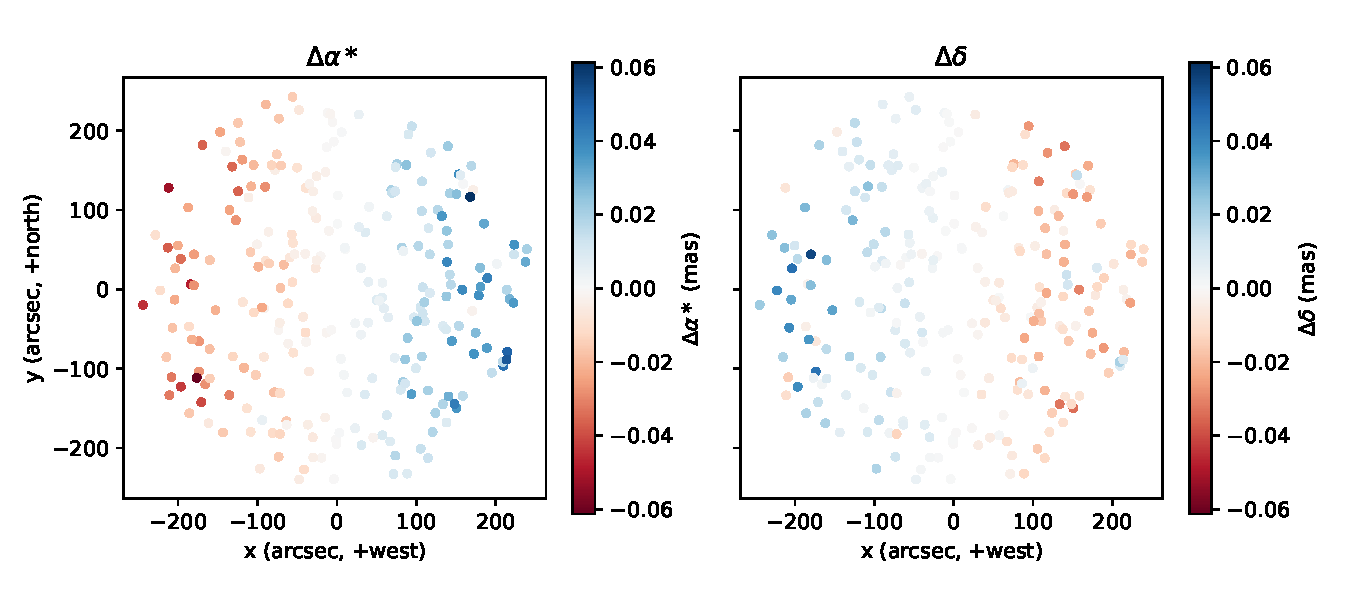
\includegraphics[width=\textwidth]{pm_propagation_map.pdf}
\caption{Position difference after \PMMapDt~yr between propagating each star's
proper motion on the sky first and propagating it unrotated in the central
tangent plane (current FlyStar), for a simulated Galactic Center field. Left:
difference along east ($\Delta\alpha*$). Right: along north ($\Delta\delta$).
After Matt Hosek's figure in GitHub issue~\#22, which used Gaia stars.}
\label{fig:pmmap}
\end{figure}

\section{Parallax}
\label{sec:parallax}

\subsection{The exact transformation}

The parallax $\varpi$ is a scalar and is the same in every projection. What
depends on the projection is the direction of the parallax displacement. A
star's apparent direction is shifted by $\varpi\,\mathbf s(t)$, where
\begin{equation}
  \mathbf s(t) = -\frac{\mathbf r_\mathrm{obs}(t) - \mathbf r_\mathrm{ref}(t)}{1\,\mathrm{au}}
  + \uvec u\left[\uvec u\cdot\frac{\mathbf r_\mathrm{obs}(t) - \mathbf r_\mathrm{ref}(t)}{1\,\mathrm{au}}\right],
  \qquad
  P_e(t) = \mathbf s\cdot\uvec e, \quad P_n(t) = \mathbf s\cdot\uvec n,
  \label{eq:pfac}
\end{equation}
with $\mathbf r_\mathrm{obs}$ the barycentric position of the observer and
$\mathbf r_\mathrm{ref}$ the barycentric position of the reference point, the
place from which $x_0$, $y_0$ are seen. This is the parallax term of the
astrometric model \citep{ESA1997, Lindegren2012}, in which the reference point
is the Solar System barycenter, $\mathbf r_\mathrm{ref} = 0$.
\code{parallax\_in\_direction} today uses the Sun,
$\mathbf r_\mathrm{ref} = \mathbf r_\odot$, so FlyStar's $x_0$, $y_0$ are
heliocentric while Gaia's are barycentric. The two differ by $\varpi$ times
the Sun's barycentric offset ($\lesssim 0.01$~au, varying over $\sim$12~yr
with Jupiter), i.e.\ $\lesssim 10$~\muas\ for $\varpi = 1$~mas. Over a few
years most of that is absorbed into the fitted proper motion, but it is a real
inconsistency with the Gaia reference stars and with Gaia's definition of the
astrometric parameters. $(P_e, P_n)$ are the east and north parallax factors
that \code{parallax\_in\_direction} computes at a given \code{(ra, dec)}. The
displacement on the sky is $\varpi(P_e,P_n)$ along the \emph{star's own} east
and north, so in the plane it maps through the same Jacobian as a proper motion:
\begin{equation}
  \begin{pmatrix} p_x \\ p_y \end{pmatrix}
  = \begin{pmatrix} -1 & 0 \\ 0 & 1 \end{pmatrix} J
    \begin{pmatrix} P_e \\ P_n \end{pmatrix}
  \approx
  \begin{pmatrix} -P_e\cos\phi + P_n\sin\phi \\ \ \ P_e\sin\phi + P_n\cos\phi\end{pmatrix},
  \label{eq:pin}
\end{equation}
where the last form is \code{parallax\_in\_direction}'s rotation by its
\code{pa} argument, $\phi$. Comparing with Eq.~\eqref{eq:jrot}, the
gnomonic frame needs $\phi = \mathrm{pa}_i = -\theta_i \approx \Delta\alpha_i\sin\delta_0$
(the frame's $+y$ axis is at $-\theta$ from the star's local north), while the
flat frame needs $\mathrm{pa}_i = 0$ (its $\cos\delta_0/\cos\delta$ scale of
$P_e$ is a part in $10^4$ at 1$'$ and can be ignored).

\paragraph{Now.} The Parallax model uses $(P_e,P_n)$ at the field center with
$\mathrm{pa}=0$ for every star, and $\mathbf r_\mathrm{ref} = \mathbf r_\odot$.
A star elsewhere in the field has a slightly different parallax ellipse
(because its $\uvec e$, $\uvec n$ differ) and, in a gnomonic frame, that
ellipse is also rotated by $\theta$. The error in the modeled displacement is
of order $\varpi$ times the offset in radians: at most \ErrMapPiMax~\muas\ for
$\varpi = \PiRef$~mas within $250''$ of the Galactic Center
(Figure~\ref{fig:errmaps}). Ingestion copies $\varpi$ correctly;
\code{project\_gaia} omits the parallax displacement altogether, which for a
Gaia star with $\varpi = 1$~mas is an error of up to 1~mas in each starlist.

\paragraph{Proposed.}
\begin{itemize}
  \item \emph{Reference point: the barycenter.} Set
    $\mathbf r_\mathrm{ref} = 0$ in \code{parallax\_in\_direction}, i.e.\
    use $-\mathbf r_\mathrm{obs}$ in place of
    $\mathbf r_\odot - \mathbf r_\mathrm{obs}$ (one line in
    \code{flystar/parallax.py}). $x_0$, $y_0$ then mean the same thing as
    Gaia's \code{ra}, \code{dec}: the direction from the barycenter at
    \code{t0}. This affects every Parallax fit, not only Gaia-based ones
    (Section~\ref{sec:proposal}).
  \item \emph{Keep the center's parallax factor.} The error from using the
    center's $(P_e,P_n)$ for every star is about a \muas\ per mas of parallax
    over a $250''$ field, well below the measurement errors, so the fitted
    $\varpi$ is kept as is in \code{prepare\_gaia\_for\_flystar},
    \code{project\_gaia} and the new utility, and nothing is refitted. If a
    much larger field ever needs it, Eq.~\eqref{eq:pin} shows how to pass
    per-star \code{ra}, \code{dec} and \code{pa} to the existing model.
  \item \emph{Include the displacement when propagating.} In
    \code{project\_gaia}, optionally add $\varpi\,\mathbf s(t)$ in
    Eq.~\eqref{eq:prop} when a precise epoch is supplied. Unlike the
    parallax-factor approximation, this omission is as large as $\varpi$.
\end{itemize}

\section{Uncertainties}
\label{sec:errors}

Positions, proper motions and parallax displacements all pass through $J$, so
their covariances transform as $C' = J\,C\,J^{\mathsf T}$ (with the sign flip of
Eq.~\eqref{eq:xy}). For gnomonic frames $J$ is a rotation by $\theta$ to
within $\rho^2$, so the error bars change only by mixing $x$ and $y$ at the
$\theta\sim10^{-4}$ level; the main error fix is the $\sigma_{x_0}$ bug of
Section~\ref{sec:now}. Gaia supplies correlations (\code{ra\_dec\_corr},
\code{pmra\_pmdec\_corr}, \code{ra\_pmra\_corr}, \dots); FlyStar's tables carry
only diagonal errors, so ingestion keeps the square roots of the diagonal of
$C'$ and the utility assumes zero correlation unless the fit's covariance is
stored.

\section{How large the differences are}
\label{sec:magnitude}

Table~\ref{tab:mag} and Figure~\ref{fig:diff} use a star offset equally east
and north of the center. The proper-motion error is for a
\PMRef~mas\,yr$^{-1}$ motion, and the parallax error is the largest difference
over a year in the modeled parallax displacement for a \PiRef~mas parallax.

\begin{table}[htbp]
\centering
\caption{Differences between the flat projection and a true gnomonic
projection, and the errors from using the center's axes for every star.}
\label{tab:mag}
\begin{tabular}{llrrrr}
\toprule
$\delta_0$ & Offset & Position & North rotation & PM error & Parallax error \\
 & & (mas) & (arcsec) & ($\mu$as\,yr$^{-1}$) & ($\mu$as) \\
\midrule
$-29^\circ$ & 10$''$ & 0.15 & 3.92 & 0.095 & 0.0488 \\
 & 1$'$ & 5.41 & 24 & 0.57 & 0.293 \\
 & 5$'$ & 135 & 118 & 2.85 & 1.46 \\
 & 30$'$ & 4{,}865 & 706 & 17 & 8.79 \\
\midrule
$+0^\circ$ & 10$''$ & $<0.001$ & 0 & 0 & 0.045 \\
 & 1$'$ & 0.00161 & 0 & 0 & 0.27 \\
 & 5$'$ & 0.201 & 0 & 0 & 1.35 \\
 & 30$'$ & 43 & 0 & 0 & 8.09 \\
\midrule
$+30^\circ$ & 10$''$ & 0.156 & 4.08 & 0.099 & 0.0292 \\
 & 1$'$ & 5.63 & 24 & 0.594 & 0.175 \\
 & 5$'$ & 141 & 122 & 2.97 & 0.876 \\
 & 30$'$ & 5{,}072 & 735 & 18 & 5.24 \\
\midrule
$+60^\circ$ & 10$''$ & 0.469 & 12 & 0.297 & 0.00572 \\
 & 1$'$ & 17 & 73 & 1.78 & 0.0343 \\
 & 5$'$ & 422 & 367 & 8.91 & 0.171 \\
 & 30$'$ & 15{,}202 & 2{,}205 & 53 & 1.01 \\
\bottomrule
\end{tabular}

\end{table}

\begin{figure}[htbp]
\centering
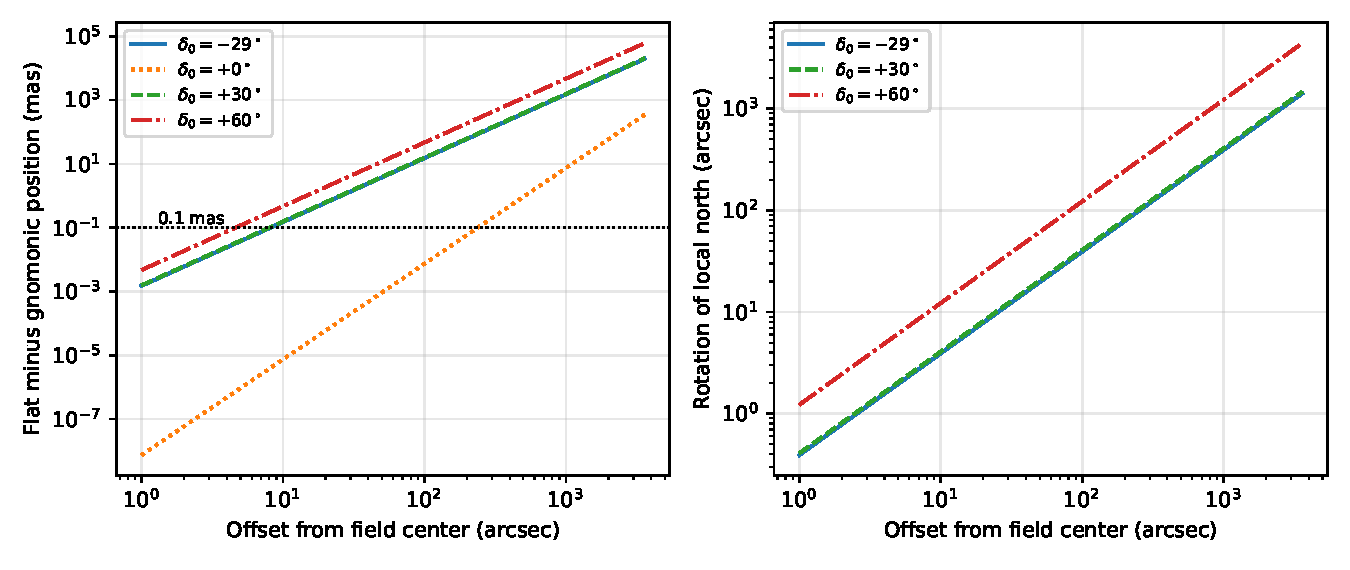
\includegraphics[width=\textwidth]{projection_differences.pdf}
\caption{Left: position difference between the flat and gnomonic projections
against offset from the field center; the dotted line marks 0.1~mas. Right:
rotation of a star's local north in the tangent plane. At $\delta_0 = 0$ the
meridians project as parallel straight lines and the rotation is zero, so that
curve is absent. The $-29^\circ$ and $+30^\circ$ curves nearly overlap because
$|\tan\delta_0|$ is similar for the two.}
\label{fig:diff}
\end{figure}

Figure~\ref{fig:errmaps} shows the same three errors star by star for the
simulated Galactic Center field of Figure~\ref{fig:pmmap}, at a single
instant, split into east and north components:
\begin{itemize}
  \item \emph{Position} (top): flat minus gnomonic, from
    Eqs.~\eqref{eq:flat} and~\eqref{eq:gnom}. The east error follows
    $\Delta\alpha\,\Delta\delta\sin\delta_0$ (opposite signs in alternate
    quadrants), and the north error follows
    $\tfrac12\Delta\alpha^2\sin\delta_0\cos\delta_0$ (same sign east and west).
    It reaches \ErrMapPosMaxInner~mas within $200''$ and \ErrMapPosMax~mas at
    $250''$.
  \item \emph{Proper motion} (middle): the plane motion FlyStar uses today
    ($J=I$) minus the correct $J_\mathrm{g}\boldsymbol\mu$
    (Eq.~\ref{eq:jgnom}), for each star's simulated proper motion. Up to
    \ErrMapPMMaxInner~\muas\,yr$^{-1}$ within $200''$ (\ErrMapPMMax\ overall).
    Multiplied by \PMMapDt~yr this is Figure~\ref{fig:pmmap} with the opposite
    sign; \code{make\_figures.py} checks that they agree.
  \item \emph{Parallax} (bottom): the largest difference over a year between
    the displacement the Parallax model assumes today (the center's factor,
    $\mathrm{pa}=0$) and the true one (the star's own factor mapped through
    $J_\mathrm{g}$, Eq.~\ref{eq:pin}), for $\varpi = \PiRef$~mas. The east
    error grows with east--west offset and the north error with north--south
    offset, reaching \ErrMapPiMaxInner~\muas\ within $200''$
    (\ErrMapPiMax~\muas\ overall). It scales linearly with $\varpi$.
\end{itemize}

\begin{figure}[htbp]
\centering
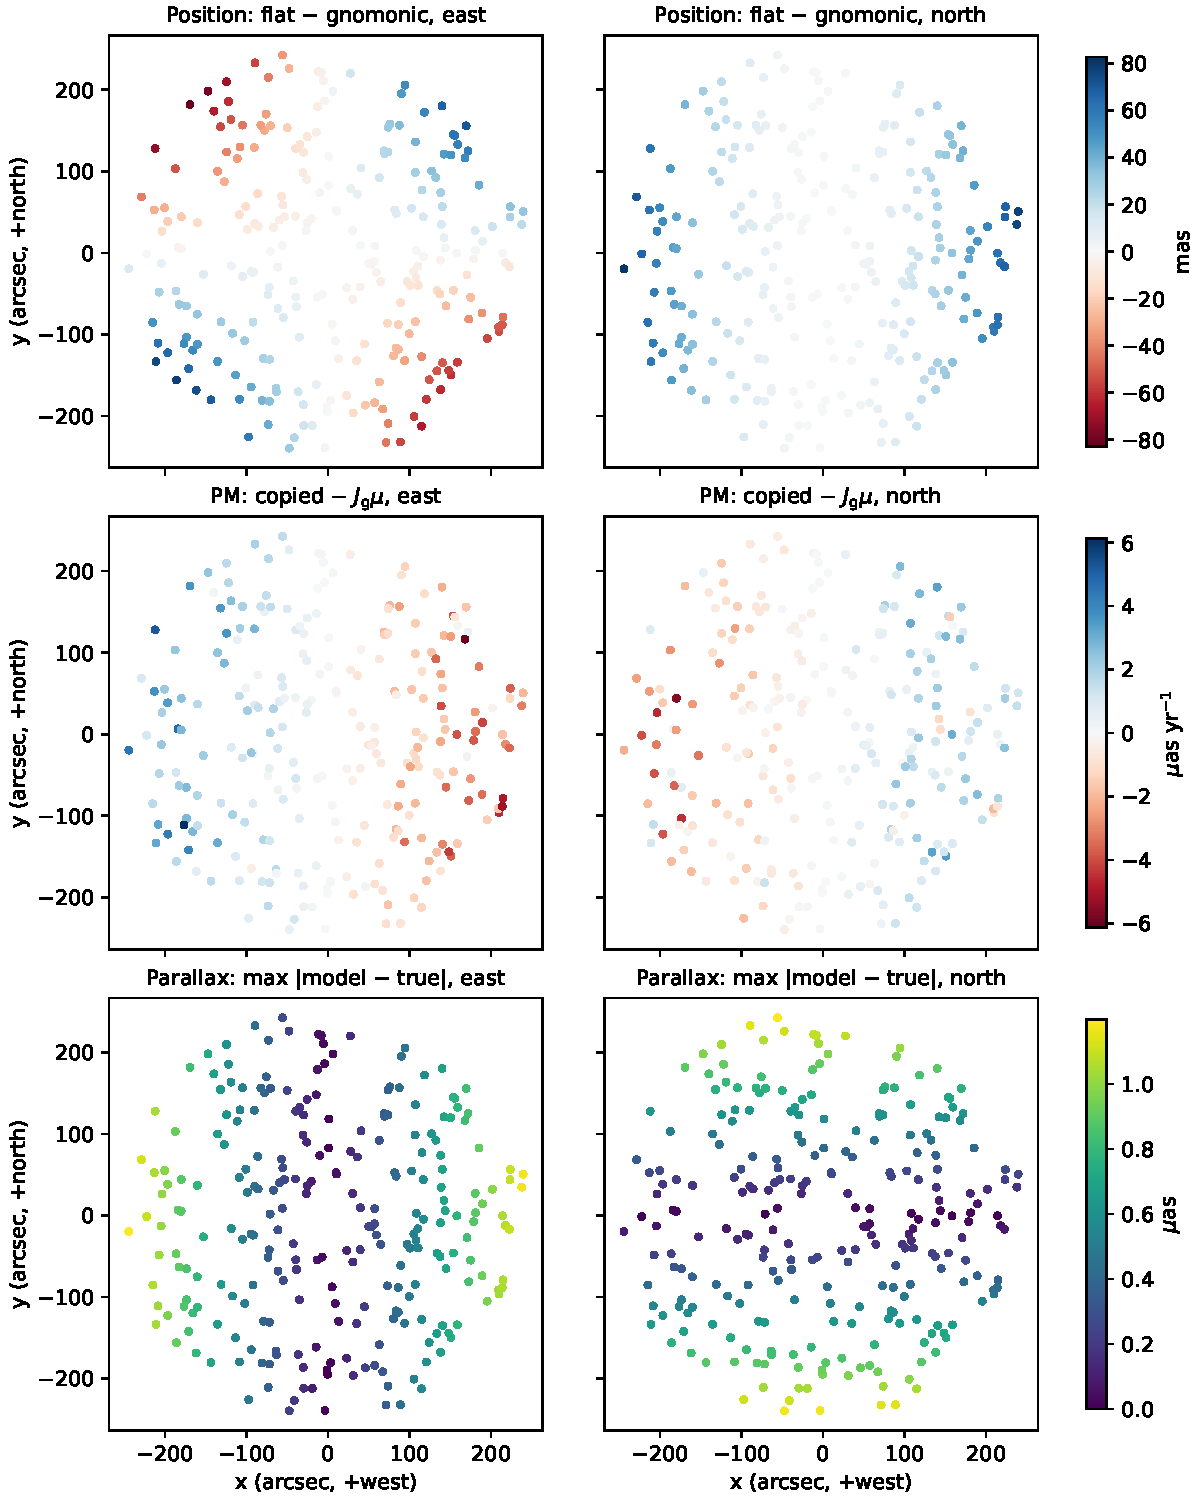
\includegraphics[width=0.85\textwidth]{error_maps.pdf}
\caption{Errors from today's handling, star by star, for the simulated
Galactic Center field of Figure~\ref{fig:pmmap} ($\delta_0 = -29^\circ$).
Left: east component. Right: north component. Top: instantaneous position,
flat minus gnomonic projection. Middle: proper motion copied into the frame
unchanged minus the correct $J_\mathrm{g}\boldsymbol\mu$. Bottom: largest
difference over one year between the parallax displacement modeled with the
field center's parallax factor and the star's true displacement in the
gnomonic frame, for a \PiRef~mas parallax. $+x$ is west, so east is on the
left.}
\label{fig:errmaps}
\end{figure}

In short:
\begin{itemize}
  \item \textbf{Positions.} For adaptive-optics fields ($\lesssim 10''$) the
    difference is about \PosDiffGCTen~mas at the Galactic Center, near the
    measurement noise. At 1$'$ it is \PosDiffGCArcmin~mas at
    $\delta_0=-29^\circ$ and \PosDiffHiArcmin~mas at $+60^\circ$, well above
    typical errors for HST or wide mosaics. Because the difference is
    quadratic in position, a second-order polynomial transformation absorbs
    most of it during alignment; first-order (affine) transformations do not.
  \item \textbf{Proper motions.} The direction error is small in absolute
    terms: \PMErrGCArcmin~\muas\,yr$^{-1}$ at 1$'$ from the Galactic Center for a
    \PMRef~mas\,yr$^{-1}$ motion, though it grows with field size and speed.
  \item \textbf{Reference stars over time.} Propagating catalog proper motions
    unrotated in the central plane moves reference stars by up to
    \PMMapMaxInner~mas within $200''$ over \PMMapDt~yr at the Galactic Center
    (Section~\ref{sec:order}).
  \item \textbf{Parallax.} Using the center's parallax direction costs about
    \PiErrGCArcmin~\muas\ at 1$'$ for a \PiRef~mas parallax, negligible for
    current fields but not for degree-scale ones; we accept it
    (Section~\ref{sec:parallax}). Omitting the parallax displacement in
    \code{project\_gaia} is far larger: up to $\varpi$ itself.
\end{itemize}

\section{Summary: now versus proposed}
\label{sec:summary}

\begin{table}[H]
\centering
\small
\caption{Current and proposed handling. $J$ is $J_\mathrm{g}$
(Eq.~\ref{eq:jgnom}) or $J_\mathrm{f}$ (Eq.~\ref{eq:jflat}) to match
\code{projection}; $F = \mathrm{diag}(-1,1)$ flips east to west.}
\label{tab:summary}
\begin{tabularx}{\textwidth}{@{}l>{\raggedright\arraybackslash}X>{\raggedright\arraybackslash}X@{}}
\toprule
Quantity & Now & Proposed \\
\midrule
Positions in & Flat (Eq.~\ref{eq:flat}) only &
  \code{'gnomonic'} (Eq.~\ref{eq:gnom}, default), \code{'flat'} (Eq.~\ref{eq:flat}), or \code{'flat\_legacy'} (today's code; temporary) \\
Position errors in & $\sigma_{x_0} = \sigma_{\alpha*}\cos\delta_0$ (bug) in \code{prepare\_gaia\_for\_flystar} &
  $C' = FJ\,C\,J^{\mathsf T}F$; $\sigma_{x_0} \approx \sigma_{\alpha*}$ \\
Proper motions in & $(v_x,v_y) = (-\mu_{\alpha*}, \mu_\delta)$ &
  $(v_x,v_y) = FJ\boldsymbol\mu$ (Eq.~\ref{eq:pmin}) \\
Bright-star PMs & As published & Optional \citet{CantatGaudin2021} correction, $G \le 13$ \\
Propagation (\code{project\_gaia}) & In the plane, unrotated; no parallax &
  On the sky, then project (Eq.~\ref{eq:prop}); optional parallax; Gaia correlations in errors \\
Parallax in & Copied & Copied (unchanged) \\
Parallax reference point & Sun (heliocentric) & Solar System barycenter \\
Parallax factor in fit & Center's $(P_e,P_n)$, $\mathrm{pa}=0$ &
  Unchanged (error $\sim$1~\muas\ per mas of $\varpi$) \\
Metadata & None &
  \code{projection}, \code{proj\_ra0}, \code{proj\_dec0}, \code{frame='icrs'}, catalog and epoch \\
Positions out & Not available & Eq.~\ref{eq:gnominv} or~\ref{eq:flatinv}, plus spherical offsets from the reference \\
Proper motions out & Not available & $\boldsymbol\mu = J^{-1}F(v_x,v_y)^{\mathsf T}$ (or Eq.~\ref{eq:pmout}) \\
Parallax out & Not available & Fitted $\varpi$, unchanged \\
\bottomrule
\end{tabularx}
\end{table}

\section{Proposed changes}
\label{sec:proposal}

\subsection{A shared projection module}

All of the equations above should live in one place (e.g.\ \code{flystar/projection.py})
so that ingestion and the utility cannot drift apart:
\begin{verbatim}
sky_to_plane(ra, dec, ra_ref, dec_ref, projection='gnomonic')
    # -> xi, eta: arcsec, east and north standard coordinates
plane_to_sky(xi, eta, ra_ref, dec_ref, projection='gnomonic')
    # -> ra, dec (deg), dlon, dlat: spherical offsets (arcsec)
jacobian(ra, dec, ra_ref, dec_ref, projection='gnomonic')   # -> J, (N, 2, 2)
propagate_on_sky(ra, dec, pmra, pmdec, dt, parallax=None, s=None)
correct_bright_pm(ra, dec, pmra, pmdec, gmag)               # -> pmra, pmdec
\end{verbatim}
The reference $(\alpha_\mathrm{ref},\delta_\mathrm{ref})$ is the projection
center (tangent point), $(\alpha_0,\delta_0)$ above.
\code{sky\_to\_plane} returns the standard coordinates of the chosen
projection about the reference, in arcsec, east and north positive: $(\xi,\eta)$
of Eq.~\eqref{eq:gnom} for gnomonic, $(\xi_\mathrm{f},\eta_\mathrm{f})$ of
Eq.~\eqref{eq:flat} for the flat modes. The callers apply $x = -\xi$.
\code{plane\_to\_sky} inverts the projection with Eq.~\eqref{eq:gnominv}
or~\eqref{eq:flatinv} and returns RA and Dec together with spherical offsets
from the reference: the longitude and latitude, east and north positive, in
a frame rotated so that the reference is at the origin, which is what
astropy's \code{SkyOffsetFrame} and \code{SkyCoord.spherical\_offsets\_to}
return \citep{Astropy2022}.

\paragraph{Caveats on this design.} We see no reason not to do it this way,
but three things should be written into the docstrings:
\begin{itemize}
  \item \emph{The offsets do not round-trip.} \code{plane\_to\_sky} applied
    to the output of \code{sky\_to\_plane} returns the same RA and Dec, but
    its spherical offsets are not the $(\xi,\eta)$ that went in. They differ
    at third order in the distance from the reference: by up to
    \SphOffOne~mas at 1$'$, \SphOffFive~mas at 5$'$ and \SphOffThirty~mas at
    30$'$ (gnomonic). So spherical offsets must not be compared with \code{x0},
    \code{y0} or passed back into \code{sky\_to\_plane} inputs; RA and Dec are
    the quantities that round-trip.
  \item \emph{Proper motions stay along local east and north.} The offset
    frame's axes at a star are rotated from that star's own east and north by
    about the angle $\theta$. Proper motions should be reported as Gaia does,
    $(\mu_{\alpha*},\mu_\delta)$ in each star's own axes, not along the offset
    axes.
  \item \emph{Spherical offsets have two common definitions.} Astropy's
    longitude offset is not multiplied by the cosine of the offset latitude;
    some authors multiply it. The difference is third order too, but the
    docstring should say which one (astropy's) we return.
\end{itemize}

\subsection{Projection modes}

\begin{itemize}
  \item \code{'gnomonic'} (default): Eq.~\eqref{eq:gnom}; proper motions
    and errors through $J_\mathrm{g}$.
  \item \code{'flat'}: Eq.~\eqref{eq:flat}; proper motions and errors
    through $J_\mathrm{f}$, with the $\sigma_{x_0}$ bug fixed. A
    self-consistent flat frame.
  \item \code{'flat\_legacy'}: today's code path, bit for bit, including
    unrotated proper motions and the $\sigma_{x_0}$ bug. For regression tests
    while the new code is written and validated; removed before release.
\end{itemize}

\subsection{\code{prepare\_gaia\_for\_flystar}}

\begin{verbatim}
prepare_gaia_for_flystar(gaia, ra, dec, targets_dict=None, match_dr_max=0.2,
                         pi_err_limit=0.4, default_motion_model='Linear',
                         projection='gnomonic', correct_bright_pm=False)
\end{verbatim}
\begin{itemize}
  \item Positions from \code{sky\_to\_plane} with the chosen projection.
  \item Proper motions from Eq.~\eqref{eq:pmin} with the matching $J$, after
    the optional bright-star correction (Section~\ref{sec:brightpm}).
  \item Errors from $C' = FJ\,C\,J^{\mathsf T}F$, fixing the $\cos\delta_0$ bug.
  \item Parallax and its error copied as now.
  \item Keep each star's \code{ra} and \code{dec} (deg) as columns, for
    matching and so that per-star parallax factors remain possible later.
  \item Write \code{projection}, \code{proj\_ra0}, \code{proj\_dec0} (deg),
    \code{frame='icrs'}, \code{parallax\_ref='ssb'}, the Gaia data release and
    whether the bright-star correction was applied to \code{meta}.
  \item Accept the center as a \code{SkyCoord}, or as numbers in degrees, with
    the current hourangle strings still accepted, so the two functions agree.
\end{itemize}

\subsection{\code{project\_gaia}}

\begin{verbatim}
project_gaia(gaia, epoch, ra, dec, projection='gnomonic',
             include_parallax=False, correct_bright_pm=False)
\end{verbatim}
\begin{itemize}
  \item Propagate on the sky with Eq.~\eqref{eq:prop}, then project with the
    chosen projection. With \code{include\_parallax=True}, \code{epoch} is
    treated as an exact decimal year and the barycentric parallax shift is
    added.
  \item Propagate errors with Gaia's correlations and $J$.
  \item Write the same metadata as \code{prepare\_gaia\_for\_flystar}.
\end{itemize}

\subsection{Parallax reference point}

Change \code{parallax\_in\_direction} to measure the observer from the
barycenter ($\mathbf r_\mathrm{ref} = 0$ in Eq.~\eqref{eq:pfac}). This is a
one-line change, but it touches every Parallax fit:
\begin{itemize}
  \item Fitted $x_0$, $y_0$ (and, through the correlation, $v_x$, $v_y$)
    shift by up to $\sim$10~\muas\ per mas of parallax relative to today's
    fits; $\varpi$ itself is essentially unchanged.
  \item Tests with hard-coded parallax vectors, and the cached vectors in
    \code{Parallax}, need updating.
  \item \code{parallax.py} was adapted from BAGLE. If FlyStar fits feed BAGLE
    models, or are compared with them, the two packages should use the same
    reference point (see Section~\ref{sec:decisions}).
  \item The table metadata records \code{parallax\_ref='ssb'} so results from
    before and after the change can be told apart.
\end{itemize}
The Parallax model's use of the center's $(P_e,P_n)$ for every star does not
change.

\subsection{Bright-star proper-motion correction}
\label{sec:brightpm}

\citet{CantatGaudin2021} found that the proper motions of Gaia (E)DR3 stars
with $G \le 13$ are rotated relative to the faint-star (quasar-defined) frame
by a magnitude-dependent spin $\boldsymbol\omega(G)$, tabulated in their paper
in bins of $G$. A spin induces the proper motion $\dot{\uvec u} =
\boldsymbol\omega\times\uvec u$, so the correction is
\begin{align}
  \mu_{\alpha*}^\mathrm{corr} &= \mu_{\alpha*} - \boldsymbol\omega\cdot\uvec n
  = \mu_{\alpha*} - \left(-\omega_x\sin\delta\cos\alpha - \omega_y\sin\delta\sin\alpha + \omega_z\cos\delta\right),
  \nonumber\\
  \mu_\delta^\mathrm{corr} &= \mu_\delta + \boldsymbol\omega\cdot\uvec e
  = \mu_\delta - \left(\omega_x\sin\alpha - \omega_y\cos\alpha\right),
  \label{eq:brightpm}
\end{align}
applied to sources with $G \le 13$ and five- or six-parameter solutions, and
left alone otherwise. Over a small field the induced motion is nearly
uniform, so it matters mainly when bright and faint reference stars are mixed:
it is then a differential motion of up to the size of the spin (tens of
\muas\,yr$^{-1}$) between the two groups. The flag
\code{correct\_bright\_pm=False} keeps today's behavior by default. The table
of $\boldsymbol\omega(G)$ applies to (E)DR3 only, so the code should check
the data release and refuse other releases until their own correction (if any)
is added.

\subsection{New utility: \code{startable\_to\_radec}}

\begin{verbatim}
radec = startable_to_radec(tab, ra_ref=None, dec_ref=None, x_ref=0.0, y_ref=0.0,
                           projection=None, scale=1.0, pa=0.0,
                           epoch=None)
\end{verbatim}
\begin{itemize}
  \item \textbf{Frame.} \code{projection}, the center and the frame default to
    the values in \code{tab.meta} written at ingestion; arguments override
    them. If \code{(x\_ref, y\_ref)} is not the projection center, the
    center's RA and Dec are solved for so that \code{plane\_to\_sky} maps
    \code{(x\_ref, y\_ref)} to \code{(ra\_ref, dec\_ref)} (a two-parameter
    Newton iteration, converging in a few steps).
  \item \textbf{Frames not from Gaia.} \code{scale} (arcsec per unit) and
    \code{pa} (deg, the position angle of $+y$ from north, as in the Parallax
    model) give $\xi = s(-x\cos\mathrm{pa} + y\sin\mathrm{pa})$ and
    $\eta = s(x\sin\mathrm{pa} + y\cos\mathrm{pa})$ for frames in pixels or not
    north-up. The defaults describe FlyStar's arcsec, north-up frame.
  \item \textbf{Positions.} \code{ra}, \code{dec} (deg, ICRS) at each star's
    \code{t0} from Eq.~\eqref{eq:gnominv} or~\eqref{eq:flatinv}; with
    \code{epoch}, propagated on the sky to a common epoch with
    Eq.~\eqref{eq:prop}.
  \item \textbf{Proper motions.} \code{pmra} ($\mu_{\alpha*}$) and
    \code{pmdec} (mas\,yr$^{-1}$) from $J^{-1}$ at each star.
  \item \textbf{Parallax.} \code{parallax} (mas) as fitted, barycentric
    for fits made after the change of reference point.
  \item \textbf{Errors.} \code{ra\_error} ($\sigma_{\alpha*}$, mas),
    \code{dec\_error}, \code{pmra\_error}, \code{pmdec\_error},
    \code{parallax\_error}, from $C' = J^{-1}F\,C\,F J^{-\mathsf T}$.
  \item \textbf{Offsets.} \code{dlon} and \code{dlat} (arcsec, east and
    north positive): the spherical offsets from \code{(ra\_ref, dec\_ref)}
    returned by \code{plane\_to\_sky}. Unlike $x_0$, these do not depend on
    any projection. The original \code{x0}, \code{y0} are kept.
\end{itemize}
Using Gaia's column names and units means the output can be fed back into
\code{prepare\_gaia\_for\_flystar}, which gives a natural round-trip test.

\subsection{Tests}
\begin{itemize}
  \item Gnomonic \code{sky\_to\_plane} against \code{astropy.wcs} with a
    \code{TAN} projection; round trips \code{plane\_to\_sky(sky\_to\_plane(.))}
    to $<1$~\muas.
  \item $J$ against numerical derivatives, and Eq.~\eqref{eq:pmout} against
    $J^{-1}$.
  \item \code{propagate\_on\_sky} against \code{SkyCoord.apply\_space\_motion}.
  \item Gaia $\to$ \code{prepare\_gaia\_for\_flystar} $\to$
    \code{startable\_to\_radec} recovers the Gaia astrometry, for both
    projections, at $\delta_0 = -29^\circ$ and $+60^\circ$ with fields up to
    $30'$.
  \item Reproduce Figure~\ref{fig:pmmap}'s difference as zero with the new
    \code{project\_gaia}.
  \item \code{'flat\_legacy'} reproduces today's outputs of both Gaia
    functions bit for bit (removed with the mode).
  \item \code{plane\_to\_sky}'s offsets against
    \code{SkyCoord.spherical\_offsets\_to}.
  \item Barycentric parallax factors against a direct calculation from
    astropy's barycentric Earth position; a fit to simulated data generated
    with Gaia's barycentric model recovers $x_0$, $y_0$ to $<1$~\muas.
  \item \code{correct\_bright\_pm} against values computed by hand from the
    spin table of \citet{CantatGaudin2021}, and leaves $G > 13$ stars unchanged.
\end{itemize}

\section{Reference frame}
\label{sec:frame}

We keep Gaia's choices: positions and proper motions in the ICRS as realized
by the Gaia catalog, the Solar System barycenter as the reference point for
parallax, a fixed projection center given in ICRS (it does not move with the
target), and each star's position at its own \code{t0}. Points to consider:
\begin{itemize}
  \item \textbf{Record, don't assume, the catalog epoch.} DR3 uses J2016.0, but
    other releases use different epochs. The code already reads
    \code{ref\_epoch} per star; the metadata should record it rather than
    hard-coding 2016.0.
  \item \textbf{ICRS, not J2000.} The center and outputs should be labeled ICRS
    throughout. A J2000/FK5 center would offset the frame by tens of mas
    \citep{FeisselMignard1998}.
  \item \textbf{Choice of center.} The projection errors grow with distance
    from the center, so the center should be near the middle of the field. If
    the science target is far from the field center, the projection center
    and the $(0,0)$ origin of $x,y$ can be different points; the metadata above
    allow this.
  \item \textbf{Barycentric reference point.} Gaia, Hipparcos and other
    astrometric missions define positions as seen from the barycenter
    \citep{ESA1997, Lindegren2012}; FlyStar will too
    (Section~\ref{sec:parallax}).
  \item \textbf{Gaia corrections.} We add the optional bright-star
    proper-motion correction (Section~\ref{sec:brightpm}). The DR3 parallax
    zero-point \citep{Lindegren2021b}, a few tens of \muas, matters for
    absolute parallaxes rather than for alignment and is not included.
  \item \textbf{Differential refraction} is corrected by KAI for Keck AO
    data before FlyStar sees it. Data from other pipelines need their own
    correction, or the transformations must absorb it.
  \item \textbf{Annual aberration} displaces every star by up to
    $\kappa = v_\oplus/c \approx 20''$, and its change across the field is a
    scale change plus a small gradient. In a field of radius 1$'$, 5$'$ and
    30$'$ the differential displacement reaches \AberRawOne, \AberRawFive\ and
    \AberRawThirty~mas. Because FlyStar fits a separate transformation for
    each epoch, nearly all of it is absorbed: what a first-order (affine)
    transformation leaves is \AberAffOne, \AberAffFive\ and
    \AberAffThirty~mas, and a second-order transformation leaves
    \AberQuadThirty~mas at 30$'$ (\code{make\_figures.py}, for the worst
    direction of the Earth's motion). So it is negligible for fields up to
    30$'$ with second-order transformations, and up to $\sim$10$'$ with
    first-order ones. Two cases break this: holding the scale fixed across
    epochs, and combining frames from different dates into one starlist
    before alignment (the scale changes by up to $\sim$$2\kappa \approx 2\times10^{-4}$
    over half a year).
\end{itemize}

\section{Decisions}
\label{sec:decisions}

\paragraph{Made.}
\begin{enumerate}
  \item \emph{Default projection:} \code{'gnomonic'}. Frames built with it
    will differ from older ones at the levels in Table~\ref{tab:mag}.
  \item \emph{Flat modes:} both \code{'flat'} (self-consistent) and
    \code{'flat\_legacy'} (bit for bit with today, for testing only, removed
    before release).
  \item \emph{Offsets:} \code{sky\_to\_plane} returns standard coordinates of
    the frame's projection about the reference in arcsec;
    \code{plane\_to\_sky} returns RA, Dec and spherical offsets.
  \item \emph{Parallax:} keep the fitted $\varpi$ and the center's parallax
    factor everywhere; no refit.
  \item \emph{Reference point:} the Solar System barycenter.
  \item \emph{Gaia corrections:} optional bright-star proper-motion
    correction, off by default; no parallax zero-point correction.
  \item \emph{Differential refraction} is handled by KAI; \emph{annual
    aberration} is absorbed by per-epoch transformations
    (Section~\ref{sec:frame}).
\end{enumerate}

\paragraph{Still open.}
\begin{enumerate}
  \item \emph{BAGLE.} Should BAGLE's parallax move to the barycenter at the
    same time, or should FlyStar's parallax module stop tracking BAGLE's?
  \item \emph{\code{include\_parallax} default} in \code{project\_gaia}. It
    needs an exact epoch, which starlists have, and it removes an error as
    large as $\varpi$; we suggest making it the default once tested.
  \item \emph{Transformation order for wide fields.} For fields beyond
    $\sim$10$'$, aberration and the flat-versus-gnomonic difference both
    argue for second-order transformations; should FlyStar warn when a wide
    field is aligned with first-order ones?
\end{enumerate}

\begin{thebibliography}{99}

\bibitem[{Astropy Collaboration}(2022)]{Astropy2022}
Astropy Collaboration, Price-Whelan, A.~M., Lim, P.~L., et al. 2022, ApJ, 935, 167.
The Astropy Project: Sustaining and growing a community-oriented open-source
project and the latest major release (v5.0) of the core package.

\bibitem[{Butkevich \& Lindegren}(2014)]{Butkevich2014}
Butkevich, A.~G., \& Lindegren, L. 2014, A\&A, 570, A62.
Rigorous treatment of barycentric stellar motion: perspective and light-time
effects in astrometric and radial velocity data.

\bibitem[{Calabretta \& Greisen}(2002)]{Calabretta2002}
Calabretta, M.~R., \& Greisen, E.~W. 2002, A\&A, 395, 1077.
Representations of celestial coordinates in FITS.

\bibitem[{Cantat-Gaudin \& Brandt}(2021)]{CantatGaudin2021}
Cantat-Gaudin, T., \& Brandt, T.~D. 2021, A\&A, 649, A124.
Characterizing and correcting the proper motion bias of the bright Gaia EDR3
sources.

\bibitem[{ESA}(1997)]{ESA1997}
ESA 1997, The Hipparcos and Tycho Catalogues, ESA SP-1200 (Noordwijk: ESA),
Vol.~1.

\bibitem[{Feissel \& Mignard}(1998)]{FeisselMignard1998}
Feissel, M., \& Mignard, F. 1998, A\&A, 331, L33.
The adoption of ICRS on 1 January 1998: meaning and consequences.

\bibitem[{Green}(1985)]{Green1985}
Green, R.~M. 1985, Spherical Astronomy (Cambridge: Cambridge University Press).

\bibitem[{Klioner et al.}(2022)]{Klioner2022}
Gaia Collaboration, Klioner, S.~A., Lindegren, L., et al. 2022, A\&A, 667, A148.
Gaia Early Data Release 3: The celestial reference frame (Gaia-CRF3).

\bibitem[{Kovalevsky \& Seidelmann}(2004)]{Kovalevsky2004}
Kovalevsky, J., \& Seidelmann, P.~K. 2004, Fundamentals of Astrometry
(Cambridge: Cambridge University Press).

\bibitem[{Lindegren et al.}(2012)]{Lindegren2012}
Lindegren, L., Lammers, U., Hobbs, D., et al. 2012, A\&A, 538, A78.
The astrometric core solution for the Gaia mission: overview of models,
algorithms, and software implementation.

\bibitem[{Lindegren et al.}(2021a)]{Lindegren2021a}
Lindegren, L., Klioner, S.~A., Hern\'andez, J., et al. 2021a, A\&A, 649, A2.
Gaia Early Data Release 3: The astrometric solution.

\bibitem[{Lindegren et al.}(2021b)]{Lindegren2021b}
Lindegren, L., Bastian, U., Biermann, M., et al. 2021b, A\&A, 649, A4.
Gaia Early Data Release 3: Parallax bias versus magnitude, colour, and position.

\bibitem[{Ma et al.}(1998)]{Ma1998}
Ma, C., Arias, E.~F., Eubanks, T.~M., et al. 1998, AJ, 116, 516.
The International Celestial Reference Frame as realized by Very Long Baseline
Interferometry.

\bibitem[{Snyder}(1987)]{Snyder1987}
Snyder, J.~P. 1987, Map Projections---A Working Manual, U.S. Geological Survey
Professional Paper 1395 (Washington: U.S. Government Printing Office).

\bibitem[{Vallenari et al.}(2023)]{Vallenari2023}
Gaia Collaboration, Vallenari, A., Brown, A.~G.~A., et al. 2023, A\&A, 674, A1.
Gaia Data Release 3: Summary of the content and survey properties.

\end{thebibliography}

\end{document}
